\documentclass[10pt]{article}
\usepackage[margin=0.72in]{geometry}
\usepackage{amsmath,amssymb,graphicx,booktabs,hyperref}
\hypersetup{colorlinks=true,urlcolor=blue}
\setlength{\parindent}{0pt}
\setlength{\parskip}{6pt}
\begin{document}
\begin{center}{\Large Guarded solving degree and regularity}\\
Rigorous degree bounds and explicit presentation controls --- 30 October 2026\end{center}

The prior scoped Lean theorem proves the exact ordinary first/last pair
$(4,5)$ for the guarded three-abscissa prime-field presentation. This
follow-up separates last fall, closed-Macaulay solving degree and the
Bardet--Faug\`ere--Salvy (BFS) degree of regularity. No exhaustive campaign
or performance measurement is reported.

\textbf{Actual inputs.} Work in $k[u,x,y,z,v]$ with
$g(T)=(T-a)(T-b)(T-c)$ and inputs
\[
 g(x),\ g(y),\ g(z),\ S_3(x,y,u),\ S_3(u,z,r),\ v(x-y)-1.
\]
For ordinary binary curves use
$S_3(s,t,w)=(st+sw+tw)^2+stw+a_6$; the guard in characteristic two is
$v(x+y)+1$. There is no implicit Boolean reduction or field equation.

\textbf{Sharp solving degree.} The original prime hypotheses are retained:
prime $p>3$, distinct base abscissas, nonsingular curve, rational target
and base lifts, and polynomial NoSolution. The prior proof constructs
$1\in V(F,5)$ and excludes it below five. For a unit ideal, a Gr\"obner
basis in $V(F,d)$ must contain a nonzero constant, by its leading-monomial
criterion applied to $1$. Conversely $\{1\}$ is a Gr\"obner basis. Lean
checks this equivalence and the exact closed solving degree five for every
monomial order. For the classical degree-compatible solving degree,
Caminata--Gorla Theorem 3.1 gives $\mathrm{sd}=\max(d_F,0)=5$.
The general bridge to a particular matrix algorithm is a cited written
corollary, not newly formalized software.

\textbf{No finite raw BFS regularity.} All six actual top forms vanish at
$(u,x,y,z,v)=(1,0,0,0,0)$, in both the prime and binary formulas. Yet
$u^d$ evaluates to $1$ for every $d\geq0$. Thus no homogeneous piece of
the top ideal is full. The finiteness assumption of BFS regularity fails.
This says nothing about infinite Castelnuovo--Mumford regularity.

\textbf{Explicit field-equation control.} Adjoining $t^q-t$ for all five
variables adds actual top forms $t^q$ for $q>1$. The previous witness
belongs to the augmented top ideal once $d\geq q$. Every monomial of
degree greater than $5(q-1)$ is divisible by a field top. Lean proves
\[ d_{\rm reg}\leq 5(q-1)+1. \]
For primes $p>3$, those field equations cannot enter a derivation below
five; the exact last fall and closed solving degree remain five after
adjoining them. The unit ideal is constructed, not assumed.

\begin{center}\small
\begin{tabular}{llll}\toprule
Presentation & Last fall & Closed solving & BFS regularity\\\midrule
Raw prime, original hypotheses & $5$ & $5$ & No finite value\\
Prime plus field equations & $5$ & $5$ & $\leq5(p-1)+1$\\
Raw ordinary binary & Not proved here & Not proved here & No finite value\\
Binary plus field equations & Not proved here & Not proved here & $\leq5(q-1)+1$\\\bottomrule
\end{tabular}\end{center}

\newpage
\begin{center}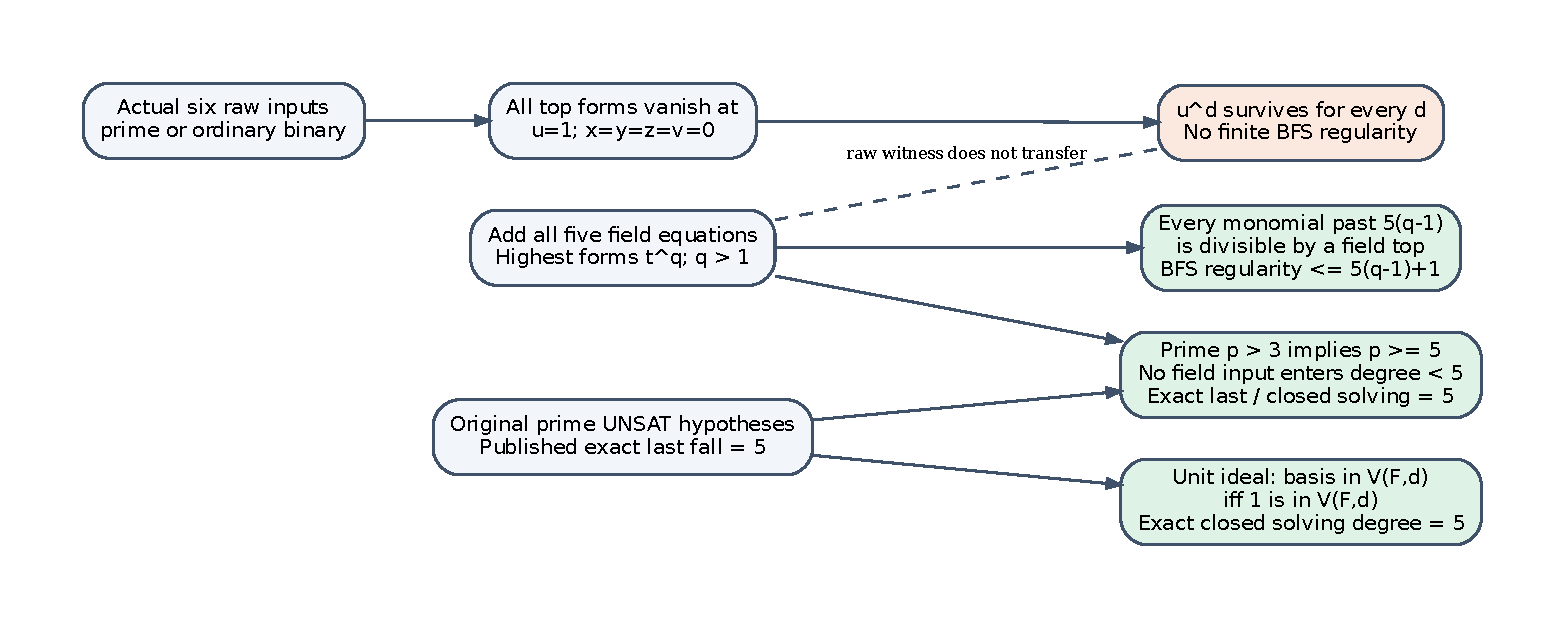
\includegraphics[width=\linewidth]{degree-invariants.pdf}\end{center}
\textit{Proof dependency diagram. All displayed bounds are mathematical
statements, not experimental measurements.}

\textbf{Formal coverage.} The added module is
\texttt{DegreeInvariants.lean}; its proof map distinguishes explicit
closure/basis definitions from the cited general classical solving-degree
bridge. Source/configuration hashes and actual default build, transitive
axiom audit and fresh kernel replay outcomes are retained separately in
\texttt{validation/}. Earlier theorem sources, hypotheses and frozen
proof-study evidence are unchanged. Failed development attempts remain
recorded separately. The complete repository library check passed 5,430 tests,
zero failed, 123 ignored; native draft-card validation passed after exact
tracked schema restoration, with the original setup failure retained.

\textbf{Exhaustive study remains open.} The designed census uses
$y^2=x^3+1$ over $\mathbb F_7$ and
$y^2+xy=x^3+x^2+1$ over
$\mathbb F_8=\mathbb F_2[t]/(t^3+t+1)$. It includes every affine target
and every three-element rational-abscissa base, with and without explicit
field equations. The bounds $31$ and $36$ for the two augmented top ideals
are proved upper bounds, not measured exact degrees.

Positive, planted-SAT, representation, A/A-permutation and changed-payload
corruption controls are specified. Complete upper/lower, basis and Hilbert
certificates are required; SAT cases cannot be assigned a last fall from a
non-contradiction or stabilization flag. No native census instrument or
canonical frozen protocol is claimed complete. AWS STS currently reports
missing credentials, and the reviewed GitHub route builds ecbench rather
than the intended instrument. No scientific run, integration-fixture
substitute or unauthorized local sweep was performed. The blocked draft
backlog card retains these obligations and has zero funding.

\textbf{Sources checked before implementation.}
Caminata--Gorla, \href{https://arxiv.org/html/2112.05579v2}{arXiv:2112.05579v2},
Definitions 1.1/1.4/1.5 and Theorem 3.1;
Semaev, \href{https://arxiv.org/html/1504.01175}{arXiv:1504.01175}, Section 2;
the existing ledger and exact-pair/top/closure Lean sources.
No novelty, asymptotic, recovery or speed claim is made.
\end{document}
